\section{Implementace}
Implementace probíhala v jazyce $C\#$ a vývojovém prostředí Unity3D \cite{Unity}, ve kterém mám dlouholetou zkušenost. 
\subsection{Základní model Boid}
Reynolds ve svém článku neuvádí jakým stylem jednotlivé pravidla řídit ani jaké váhy použít. Byla tedy vytvořena váha pro každé pravidlo, díky kterému můžeme řídit prioritu těchto pravidel. 
\par
Pro lepší vizuální představu jak model Boid funguje byl vytvořen jednoduchý editor, ve kterém je možné v reálném čase nastavit upravit váhy jednotlivým pravidlům a vidět změnu v chování hejna, aniž by bylo potřeba pouštět celou simulaci znovu. To umožnilo rychleji dosáhnout požadovaného chování hejna. Pro správné nastavení vah by teoreticky šel použít i evoluční algoritmus, avšak na tak jednoduchém příkladě není jasné jakým způsobem určovat fitness. 
\par
Podařilo se dosáhnout fungujícího modelu hejna, které však nekontrolovaně cestovalo po světě. 

\subsection{Rozšíření o pravidlo Cíl}
Model Boid popisuje pouze chování jednotlivce v hejnu. Pro potřebu kontrolovat pohyb celého hejna, byl agent rozšířen o další pravidlo. Každý agent se snaží dostat do cíle, který je reprezentován pozicí bodu ve světě. 
\par
Od toho pravidla vyžadujeme, ať přitahuje agenta k cíli, ale neznehodnotí zbylé 3 pravidla s narůstající vzdáleností od cíle. Normalizování směrového vektoru k cíli se může zdát jako krok správným směrem. V praxi se však ukázalo, že když je takový agent velmi blízko svého cíle, normalizace vektor naopak zvětší. To má za následek příliš agresivní snahu jedince dostat se do cíle. Proto velikost směrového vektoru od jedince k cíli pouze ořízneme na hodnotu vzdálenosti, od které má být agent méně agresivní. 
\par
Pomocí nového pravidla je možné kontrolovat pozici hejna a pozicovat ho dle svých potřeb. Pro názornou ukázku vznikla scéna s akváriem a rybičkami. V určitém časovém intervalu nastavuji všem agentům (rybám) náhodně vygenerovaný cíl uvnitř akvária.  
\begin{figure}[H]
	\label{fig:ryby_20_50}
	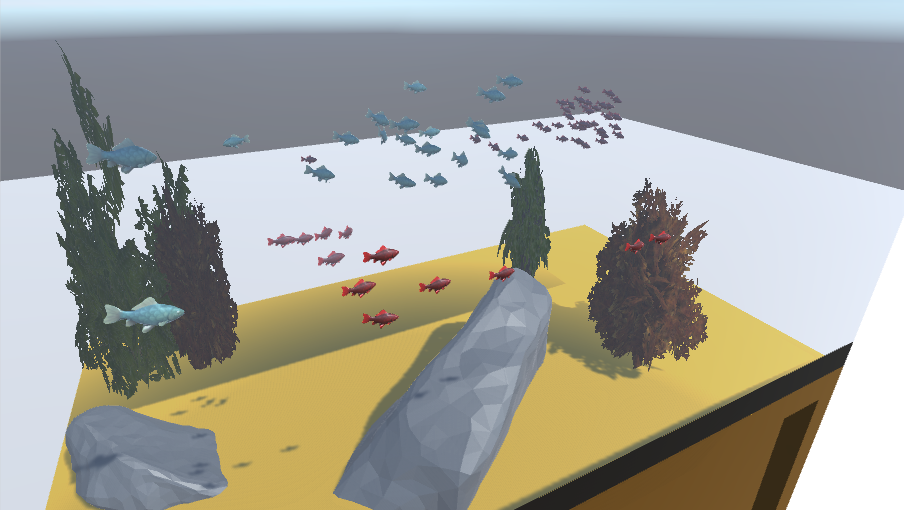
\includegraphics[width=10cm]{fish_20_50.png}
	\centering
	\caption{Hejno 20 modrých a 50 červených ryb}
\end{figure}
Na obrázku \ref{fig:ryby_20_50} můžeme vidět 2 různě početné a nastavené skupiny agentů. První je skupina 20 velkých modrých ryb, které jsou pomalé, drží se dál od sebe (velká váha u separace) a pomalu mění svůj směr. Druhá skupina obsahuje 50 malých červených ryb, které jsou rychlejší, agilnější, ale více se drží pohromadě (velká váha u koheze a vyrovnání). 
\par
Stejnými pravidly se dá simulovat i dav lidí, kteří se potřebují dostat z jednoho místa na druhé. Pro tyto účely byl každému jedinci nastaven odlišný cíl. Obrázek \ref{fig:srovnaniVahy} znázorňuje srovnání chování 2 skupin poslaných proti sobě. Červená skupina na levém obrázku má nastavené váhy pro Kohezi a Vyrovnání převyšující váhu pravidla pro Cíl. Na pravém obrázku mají nastaveny váhy pro Kohezi a Vyrovnání tak, aby součet těchto vah nepřekročil váhu pro Cíl. Modrá skupina má nastavené pouze pravidlo Separace a Cíl. Pravidla pro Kohezi a Vyrovnání mají nulovou váhu. Každý agent má za úkol dostat se na druhou stranu a zaujmout pozici v pomyslné mřížce. Obrázky ve směru dolů jsou stavem s narůstajícím časem simulace. 
\begin{figure}[H]
	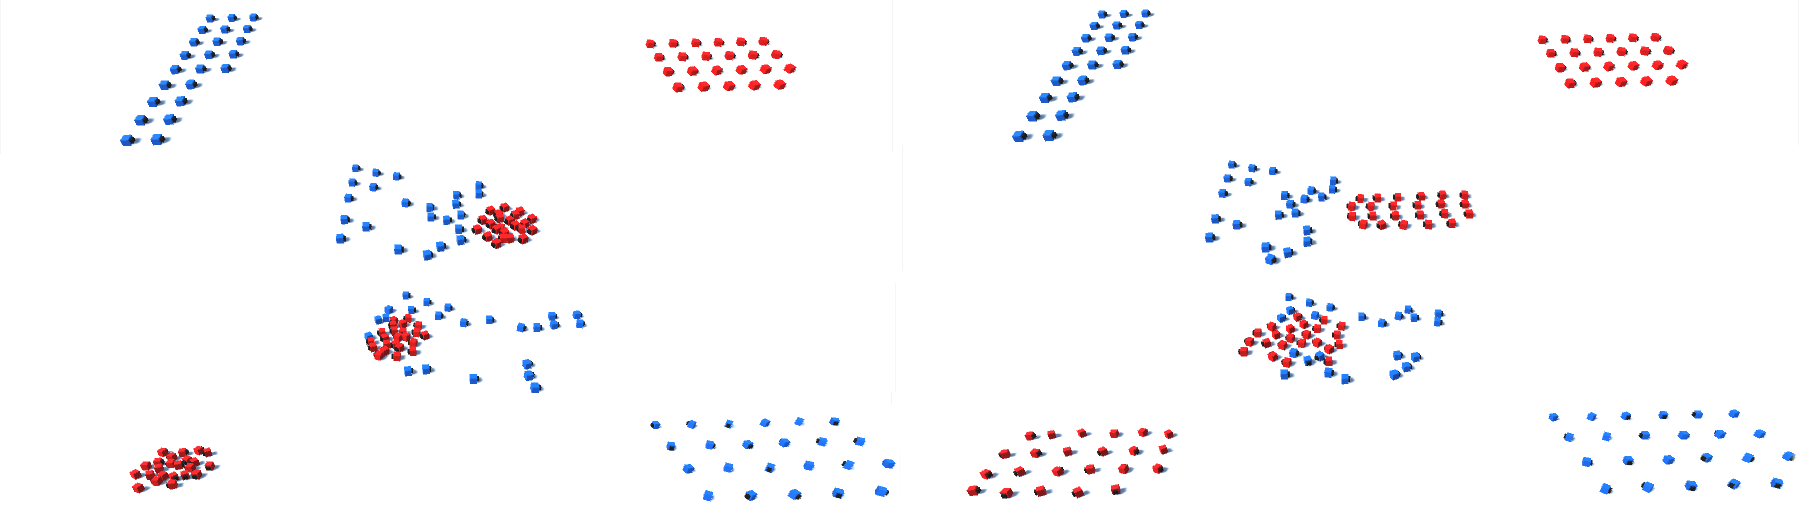
\includegraphics[width=10cm]{entities_weights.png}
	\centering
	\caption{Srovnání vah v časech $t\in\{ 0,20,30,70\} $}
	\label{fig:srovnaniVahy}
\end{figure}
Z obrázku \ref{fig:srovnaniVahy} můžeme usoudit, že poměr mezi váhou Cíle a váhami Koheze a Vyrovnání nemá na hejno jako celek vliv. V obou případech se hejno dostalo na druhou stranu. Avšak při malé váze pravidla Cíl nedokáže jedinec zaujmout svou koncovou pozici.  

\subsection{Rozšíření o pravidlo Vyhni se překážkám}
Dalším přidaným pravidlem, díky kterému bude chování hejna více připomínat realitu je uhýbání před překážkami. Každý agent si v závislosti na své rychlosti kontroluje prostor před sebou. Pokud detekuje překážku, vychýlí svůj vektor rychlosti tak, aby se pokusil překážce vyhnout. 
\begin{figure}[H]
	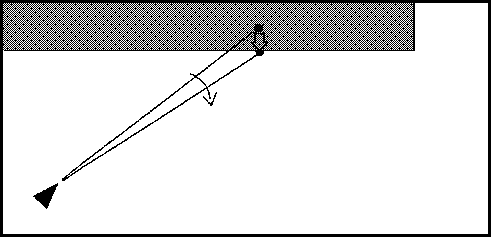
\includegraphics[width=10cm]{collisionAvoidance.png}
	\centering
	\caption{Vychýlení vektoru rychlosti při detekci překážky \cite{ReynoldsBoidNoBump} }
\end{figure}
Pro test byly do scény přidány 2 překážky a puštěna obvyklá simulace dvou skupin, která si mají vyměnit místa. Na obrázku \ref{fig:agents_anim} můžeme pozorovat, že hejno překážku obteče a má tendenci se zase spojit do jednoho shluku. 
\begin{figure}[H]
	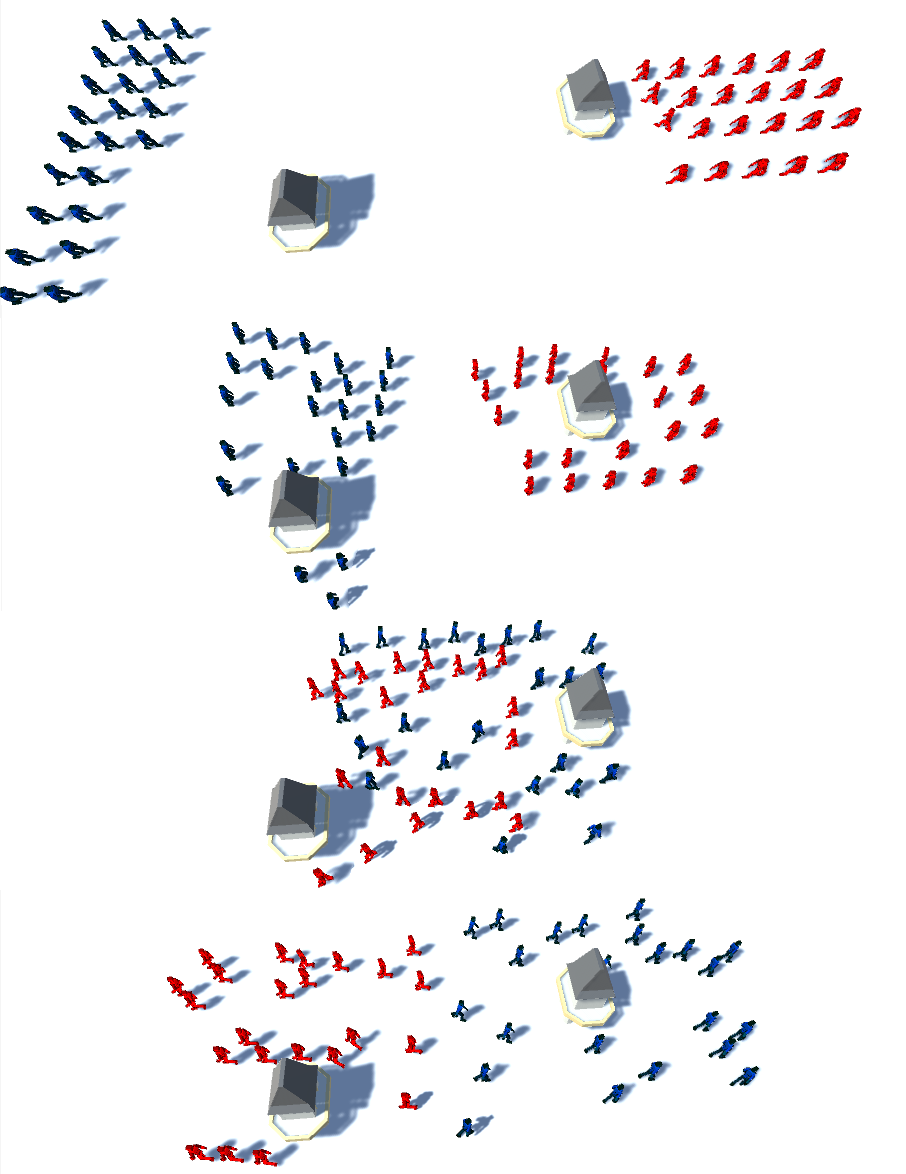
\includegraphics[width=10cm]{peopleAgents_anim.png}
	\centering
	\caption{2 skupiny agentů s detekcí překážek v časech $t\in\{ 0,10,20,30\} $}
	\label{fig:agents_anim}
\end{figure}
